\begin{frame}
    Dans cette section nous allons étudier numériquement le problème de Rayleigh-Stokes en $1$D sur le segment $[0, L]$ où $L>0$ est un réel que l'on précisera lors de l'implémentation de quelques cas tests. On va considérer le problème suivant
\begin{equation*}
\begin{cases}
    \partial_tu(t,x) - \nu\partial_{xx} u(t,x) - \alpha\partial_{xxt} u(t,x) = f & \forall (t,x) \in  \bbR_+^* \times \ ]0,L[  \\
    u(0,x) = u_0(x) & \forall x \in \ ]0,L[ \\
    u(t, 0) = u(t,L) = 0 & \forall t \in \bbR_+^*
\end{cases}
\end{equation*}
Tout comme le réel $L$, on précisera la donnée initiale $u_0$ et le second membre $f$ lors de l'implémentation des cas tests. Nous allons approcher ce problème par une méthode différence finie.
\end{frame}

\subsection{Définition du schéma différence finie}
\begin{frame}
    \begin{itemize}
        \item Commençons par la discrétisation spatiale. Soit $m \in \bbN^*$ le nombre de maille. On pose $h = \dfrac{L}{m+1}$ le pas d'espace et $x_i = ih$ les noeuds du maillage. 
        \item On approche $\partial_{xx}$ par l'opérateur approché à trois noeuds
\begin{equation*}
    \Delta_hu(t,x) = \frac{u(t,x-h)-2u(t,x)+u(t,x+h)}{h^2}
\end{equation*}
\item On note $u_h$ la solution numérique et on veut calculer cette solution aux point $x_i$, on pose $u_i(t)=u_h(t,x_i)$ et $f_i=f(x_i)$. On obtient le schéma semi-discret
\begin{equation*}\label{schema_semi_discret}
    \partial_tu_i(t)-\nu\frac{u_{i-1}(t)-2u_i(t)+u_{i+1}(t)}{h^2}-\alpha\frac{\partial_tu_{i-1}(t)-2\partial_tu_i(t)+\partial_tu_{i+1}(t)}{h^2}=f_i
\end{equation*}
\item On passe ensuite à la discrétisation temporelle. 
        \item Soit $T>0$ le temps final. On partitionne $[0,T]$ en introduisant les instants 
$t_n = n \Delta t$, où $\Delta t$ est le pas de temps. 
\item On note à présent $u_i^n=u_h(x_i,t_n)$ l'approximation de la 
solution $u(x,t)$ au point $x_i$ et à l'instant $t_n$. 
    \end{itemize}
\end{frame}

\begin{frame}
    \begin{itemize}
\item On va utiliser le schéma d'Euler implicite pour l'approximation 
temporelle.
\begin{eqnarray*}\label{schema_DF_points}
    \frac{u_i^{n+1}-u_i^n}{\Delta t} - \nu \frac{u_{i-1}^{n+1}-2u_i^{n+1}+u_{i+1}^{n+1}}{h^2} &-& \frac{\alpha}{\Delta t}\bigg( \frac{u_{i-1}^{n+1}
    -2u_i^{n+1}+u_{i+1}^{n+1}}{h^2}\\
    &-&\frac{u_{i-1}^{n}-2u_i^{n}+u_{i+1}^{n}}{h^2}\bigg) \\
    &=& f_i
\end{eqnarray*}
        \item Notons à présent $U^n$ le vecteur solution à l'instant $n$, 
$\Delta_h$ la matrice de discrétisation de la dérivée seconde en 
espace et $F$ le vecteur second membre. 
\item On peut ainsi réécrire l'équation précédente de la façon suivante
\begin{eqnarray*}
    \frac{U^{n+1} - U^n}{\Delta t} - \nu \Delta _h U^{n+1} - \alpha\bigg(\frac{\Delta_h U^{n+1} - \Delta_h U^n}{\Delta t} \bigg) = F
\end{eqnarray*}
\item En réorganisant les termes pour isoler l'inconnue au temps $n+1$, nous obtenons le système 
\begin{eqnarray}\label{schema_DF}
    \big(I - (\nu \Delta t + \alpha)\Delta_h\big)  U^{n+1} = (I - \alpha \Delta_h) U^n + \Delta t F
\end{eqnarray}
où $I$ désigne la matrice identité. On peut maintenant s'intéresser aux propriétés de ce schéma.
    \end{itemize}
\end{frame}

\subsection{Propriétés du schéma}

\begin{frame}
    \begin{itemize}
        \item Le schéma est consistant d'ordre 1 en temps et d'ordre 2 en espace. 
        \item Le facteur d'amplification de ce schéma est
        \begin{eqnarray*}
    \mathscr{A}(k \ ; \Delta t ,h) &=& \frac{1 +  4 \dfrac{\alpha}{h^2} \sin^2(\pi k h)}{1+4\dfrac{\alpha}{h^2}\sin^2(\pi k h) + 4 \dfrac{\nu \Delta t}{h^2}\sin^2(\pi k h) }
\end{eqnarray*}
Puisque $\nu, \ \Delta t > 0$ on obtient 
\begin{eqnarray*}
    \sup_{k \in \mathbb{Z}} \ |\mathscr{A}(k \ ; \Delta t ,h)| &\leq& 1
\end{eqnarray*}
Le schéma est donc stable en temps long et inconditionnellement stable en norme $L^2$. 
\item Le schéma est consistant d'ordre un en temps et deux en espace et il est
stable en norme $L^2$, donc le schéma converge. De plus, l'erreur globale est en $O(\Delta t +h^2)$.
    \end{itemize}
\end{frame}

\begin{frame}
    \begin{itemize}
        \item \'Etudions à présent le rôle de $\alpha$. On suppose que $h$ et 
$\Delta t$ sont fixés et suffisamment petit. 
\item \`A basses fréquences, on a 
\begin{equation*}
    \scrA (k \ ; \Delta t ,h) \approx 1
\end{equation*}
autrement dit, les basses fréquences sont conservées peu importe la valeur du paramètre $\alpha$. 
\item Et à hautes fréquences, on a 
\begin{equation*}
    \scrA(k \ ; \Delta t ,h) \approx \dfrac{1+\alpha\dfrac{4}{h^2}}{1+(\alpha+\nu\Delta t)\dfrac{4}{h^2}} \approx \dfrac{\alpha}{\alpha+\nu\Delta t}
\end{equation*}
\item On observe alors plusieurs cas
\begin{itemize}
    \item[$\triangleright$] si $\alpha \ll \nu \Delta t$ alors $\scrA(k \ ; \Delta t ,h) \approx 0$, les hautes fréquences sont complètement amorties ; 
    \item[$\triangleright$] si $\alpha \sim \nu \Delta t$ alors $\scrA(k \ ; \Delta t ,h) \approx \dfrac{1}{2}$, les hautes fréquences sont moyennement amorties ; 
    \item[$\triangleright$] si $\alpha \gg \nu\Delta t$ alors $\scrA(k \ ; \Delta t ,h) \approx 1$,
    les hautes fréquences sont conservées.
\end{itemize}
    \end{itemize}
\end{frame}


\begin{frame}
    Mettons en évidence cette propriété en implémentant un cas test très simple. Prenons les paramètres suivant $L=1$, $T=1$, $f\equiv 0$, $\nu=0.1$, $h=\Delta t=\dfrac{1}{100}$ et $u_0(x)=\sin(\pi x)+\sin(10\pi x)$.
\begin{figure}[!ht]
    \centering
    \begin{subfigure}{0.32\textwidth}
        \centering
        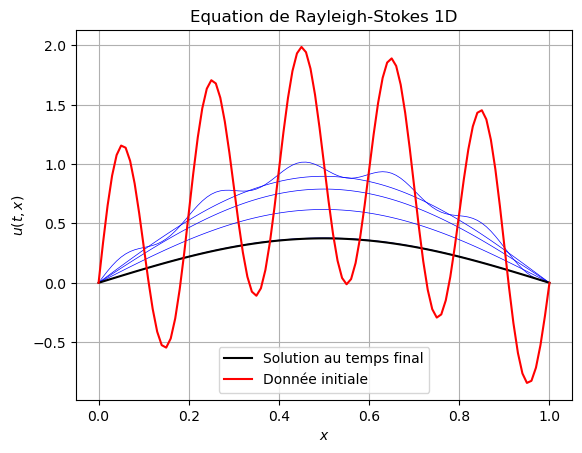
\includegraphics[width=\textwidth]{images/stabilité/alpha_dix_moins_5.png}
        \caption{$\alpha=10^{-5}$}
    \end{subfigure}
    \hfill
    \begin{subfigure}{0.32\textwidth}
        \centering
        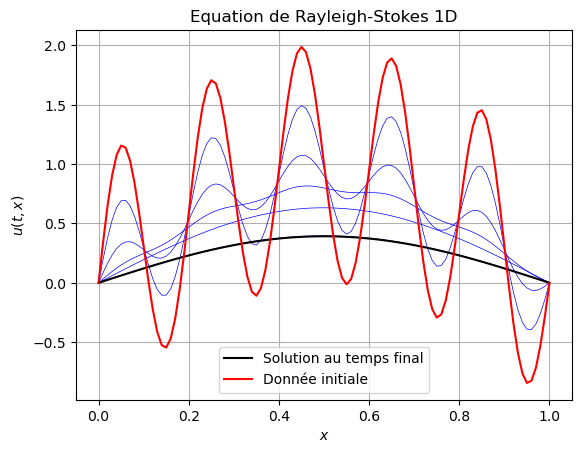
\includegraphics[width=\textwidth]{images/stabilité/alpha_dix_moins_2.png}
        \caption{$\alpha=5\times 10^{-3}$}
    \end{subfigure}
    \hfill
    \begin{subfigure}{0.32\textwidth}
        \centering
        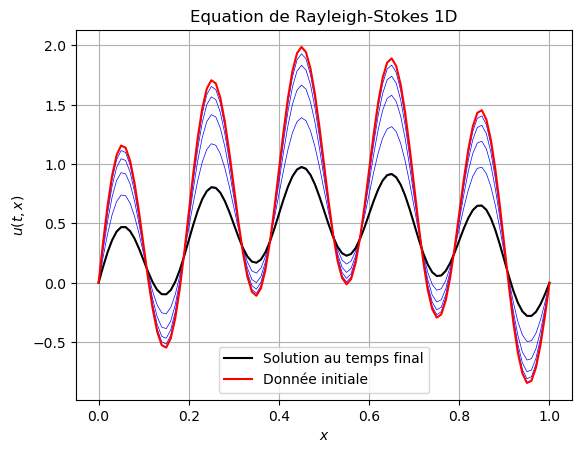
\includegraphics[width=\textwidth]{images/stabilité/alpha_dix_moins_1.png}
        \caption{$\alpha=10^{-1}$}
    \end{subfigure}
    \caption{Comportement des hautes fréquences en fonction de $\alpha$}
    \label{fig:stabilite_alpha}
\end{figure}
\end{frame}

\subsection{Un exemple}

%\begin{frame}{Créneau}
%\begin{itemize}
%\item On veut observer l'effet de régularisation de l'équation pour une donnée
%initiale discontinue.
%\item On s’intéresse donc au problème suivant
%   \begin{equation*}
%        \begin{cases}
%            \partial_tu(t,x) - \nu\partial_{xx} u(t,x) - \alpha\partial_{xx} \big(\partial_t u(t,x)\big) = 0 & \forall (t,x) \in \ ]0, T[ \ \times \ ]0,L[  \\
%            u(0,x) = u_0(x) = \mathds{1}_{\left[\tfrac{L}{4},\tfrac{3L}{4}\right]}(x) & \forall x \in \ ]0,L[ \\
%            u(t, 0) = u(t,L) = 0 & \forall t \in \ ]0,T[
%        \end{cases}
%    \end{equation*}
%    \item On résout numériquement le problème en posant 
%    $N = 200$, $L=10$ et $T=20$. Pour les paramètre de 
%    l'équation de Rayleigh-Stokes on choisi $\nu = 0.4$ et 
%    $\alpha=0.5$ Cela va nous permettre d'étudier 
%    comment varie notre solution initial et quels sont les 
%    effets du paramètre $\alpha$.
%    \end{itemize}
%\end{frame}

%\begin{frame}{Créneau}  
%\begin{figure}[!ht]
%        \centering
%        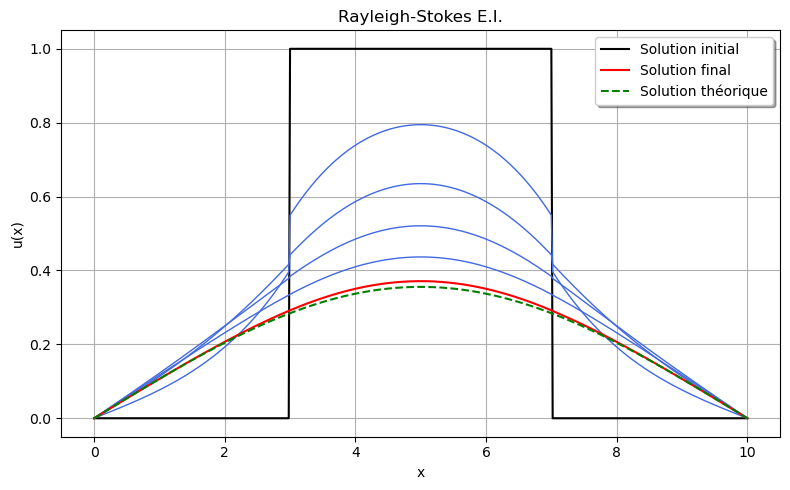
\includegraphics[width=0.6\textwidth]{images/Exemples/Indicatrice/resolution_indicatrice.png}
%    \caption{ Résolution de l'équation de Rayleigh-Stokes $1$D}
%    \label{fig:Exemples_RS_Stokes_indicatrice}
%\end{figure}
%\begin{eqnarray*}
%    u(t,x) = \sum_{k=1}^{N} \frac{2}{k\pi}\left(\cos\Big(\frac{k\pi}{4}\Big) -\cos\Big(\frac{3k\pi}{4}\Big)\right) \exp\left(-\frac{\nu\lambda_k}{1+\alpha\lambda_k}\,t\right)\sin\left(\frac{k\pi x}{L}\right)
%\end{eqnarray*}
%\end{frame}

%\begin{frame}
%    \begin{figure}[!ht]
%        \centering
%    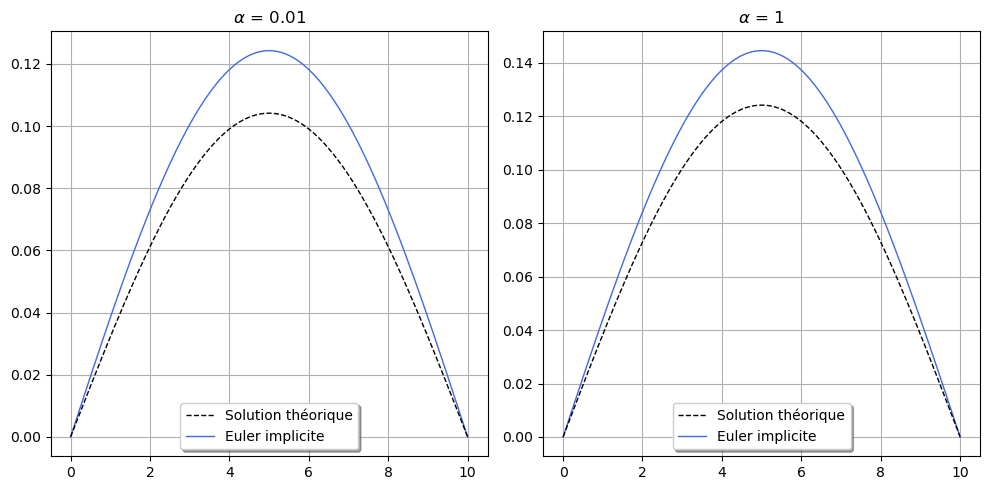
\includegraphics[width=\linewidth]{images/Exemples/Indicatrice/comparaison alpha indicatrice.png}
%    \caption{Comparaison en fonction de $\alpha$}
%    \label{Indicatrice_comparaisons des alpha}
%    \end{figure}
%\end{frame}

\begin{frame}{Problème de Stokes impulsif}
    \begin{itemize}
        \item On va maintenant simuler la réponse d'un fluide à l'accélération 
d'une paroi. 
\item Le problème s'écrit
\begin{equation*}
    \begin{cases}
        \partial_tu(t,x) - \nu\partial_{xx} u(t,x) - \alpha\partial_{xx} \big(\partial_t u(t,x)\big) = 0 & \forall (t,x) \in \ ]0, 5[ \ \times \ ]0,1[  \\
        u(0,x) = u_0(x) = 0 & \forall x \in \ ]0,1[ \\
        u(t,1) = 0 & \forall t \in \ ]0,5[ \\
        u(t,0) = U_0:=10 & \forall t \in \ ]0,5[
    \end{cases}
\end{equation*}
    \end{itemize}
\end{frame}

\begin{frame}{Problème de Stokes impulsif}
    \begin{figure}[!ht]
    \centering
    \begin{subfigure}{0.32\textwidth}
        \centering
        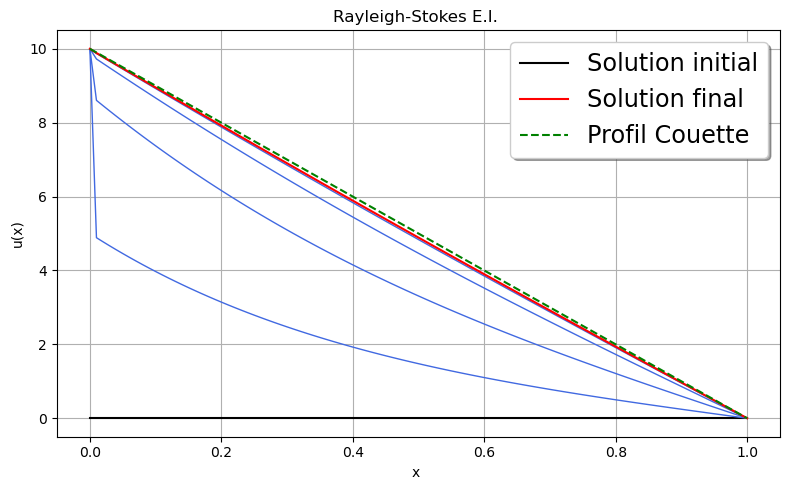
\includegraphics[width=\textwidth]{images/Exemples/Plaque en mouvement/RS_EI_plaque_1.png}
        \caption{$\alpha=0.1$}
    \end{subfigure}
    \hfill
    \begin{subfigure}{0.32\textwidth}
        \centering
        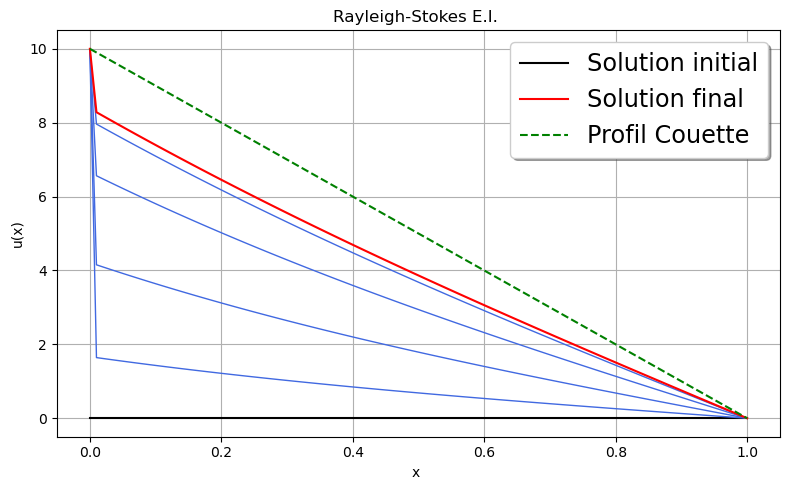
\includegraphics[width=\textwidth]{images/Exemples/Plaque en mouvement/RS_EI_plaque_2.png}
        \caption{$\alpha=0.5$}
    \end{subfigure}
    \hfill
    \begin{subfigure}{0.32\textwidth}
        \centering
        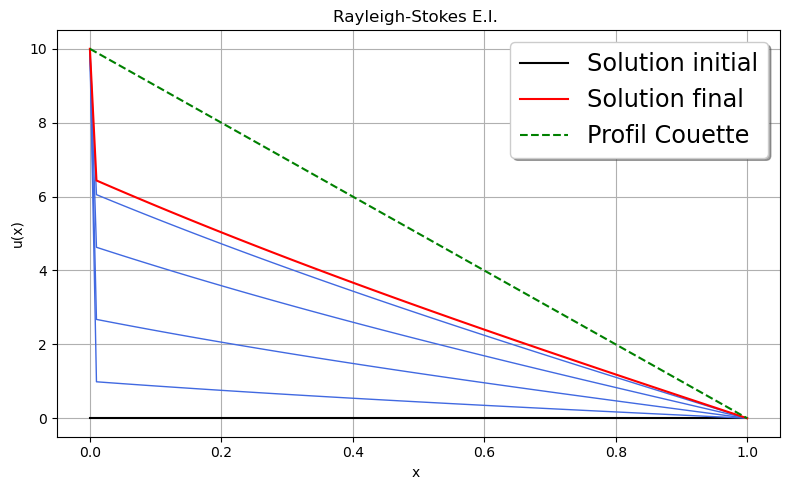
\includegraphics[width=\textwidth]{images/Exemples/Plaque en mouvement/RS_EI_plaque_3.png}
        \caption{$\alpha=0.9$}
    \end{subfigure}
    \caption{Influence du paramètre $\alpha$ sur la résistance du fluide face à la condition initiale pour l'équation de Rayleigh-Stokes $1$D}
    \label{fig:Exemples_RS_Stokes_impulsif}
\end{figure}
\end{frame}

\subsection{Comparaison avec l'équation de la chaleur}

\begin{frame}
    \begin{itemize}
    \item Problème aux limites pour l'équation de Rayleigh-Stokes
    \begin{equation*}
        \begin{cases}
            \partial_tu(t,x) - \nu\partial_{xx} u(t,x) - \alpha\partial_{xx} \big(\partial_t u(t,x)\big) = 0 & \forall (t,x) \in \ ]0, 1[ \ \times \ ]0,1[  \\
            u(0,x) = u_0(x) = \sin{(\pi x)} & \forall x \in \ ]0,1[ \\
            u(t, 0) = u(t,1) = 0 & \forall t \in \ ]0,1[
        \end{cases}
    \end{equation*}
    \item Problème aux limites pour l'équation de la chaleur
    \begin{equation*}
        \begin{cases}
            \partial_tu(t,x) - \nu\partial_{xx} u(t,x) = 0 & \forall (t,x) \in \ ]0,1[ \ \times \ ]0,1[  \\
            u(0,x) = u_0(x)=\sin{(\pi x)} & \forall x \in \ ]0,1[ \\
            u(t, 0) = u(t,1) = 0 & \forall t \in \ ]0,1[
        \end{cases}
    \end{equation*} 
    \item Les solutions de ces problèmes sont 
    \begin{eqnarray*}
        u_{\text{RS}}(t,x) = \sin{(\pi x)}\exp{\Big( -\frac{\nu \pi^2}{1+\alpha \pi^2}t\Big)}
        &\text{ et }& u_{\text{chal}}(t,x) = \sin{(\pi x)}\exp{(-\nu \pi^2t)}
    \end{eqnarray*}
\end{itemize}
\end{frame}

\begin{frame}
    \begin{itemize}
        \item L'objectif ici est d'observer l'influence du paramètre $\alpha$ sur la dissipation de l'énergie cinétique et de comparer ce phénomène avec l'équation de la chaleur (cas $\alpha=0$). 
        \item Pour nos simulations, on choisit $\nu = 0.1$, et $h=\Delta t = \dfrac{1}{100}$. La simulation pour l'équation de la chaleur donne le résultat suivant
\begin{figure}[!ht]
    \centering
    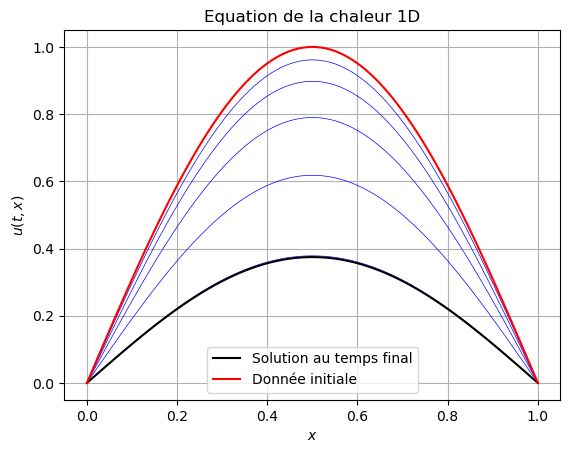
\includegraphics[width=0.5\linewidth]{images/comparaison_chaleur/eq_chaleur.png}
    \caption{\'Equation de la chaleur $1$D pour l'évolution temporelle du profil de vitesse $u(t,x)$ pour un mode sinusoïdal}
    \label{fig:eqchaleur}
\end{figure}
    \end{itemize}
\end{frame}

\begin{frame}
    \begin{itemize}
        \item Pour comparer à l'équation de Rayleigh-Stokes, on choisit $\alpha \in \{5\times 10^{-1}, 5 \times 10^{-2}, 5 \times 10^{-4}\}$. 
    \end{itemize}
        \begin{figure}[!ht]
    \centering
    \begin{subfigure}{0.32\textwidth}
        \centering
        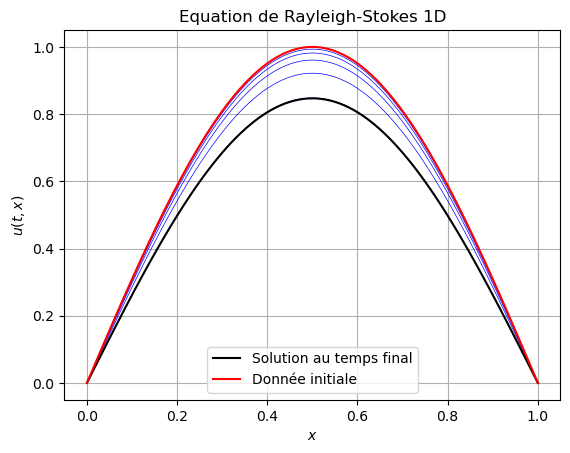
\includegraphics[width=\textwidth]{images/comparaison_chaleur/eq_RS_alpha1.png}
        \caption{$\alpha=5\times 10^{-1}$}
    \end{subfigure}
    \hfill
    \begin{subfigure}{0.32\textwidth}
        \centering
        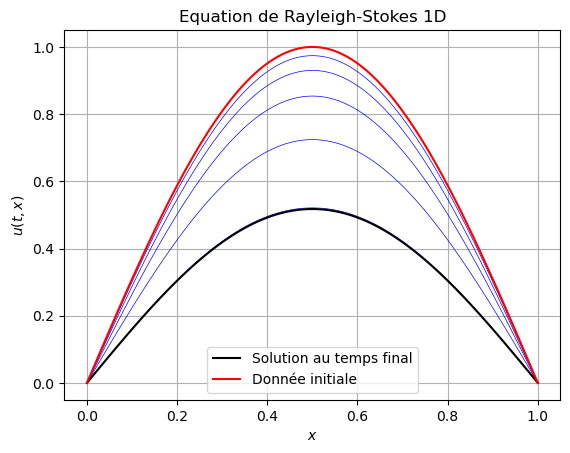
\includegraphics[width=\textwidth]{images/comparaison_chaleur/eq_RS_alpha2.png}
        \caption{$\alpha=5\times 10^{-2}$}
    \end{subfigure}
    \hfill
    \begin{subfigure}{0.32\textwidth}
        \centering
        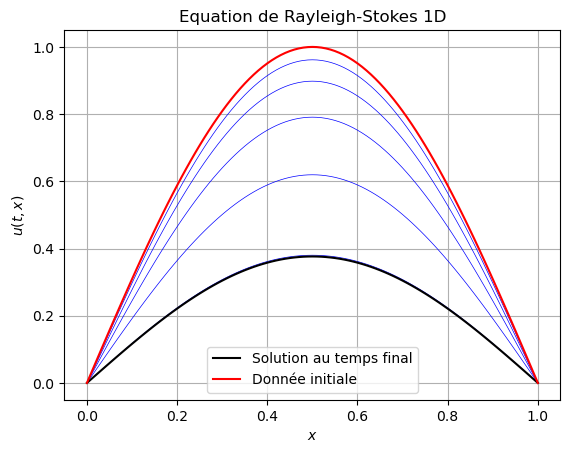
\includegraphics[width=\textwidth]{images/comparaison_chaleur/eq_RS_alpha3.png}
        \caption{$\alpha=5 \times 10^{-4}$}
    \end{subfigure}
    \caption{Influence du paramètre $\alpha$ sur la dissipation de l'énergie pour l'équation de Rayleigh-Stokes $1$D}
    \label{fig:comparaisonchaleurRS}
\end{figure}
\end{frame}

%\begin{frame}{Code C++}
%    \begin{figure}[!ht]
%    \centering
%    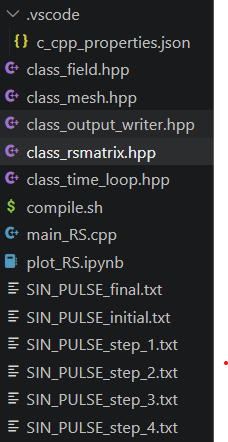
\includegraphics[width=0.25\linewidth]{images/code.png}
%    \caption{Architecture du code C++}
%    \label{fig:code}
%\end{figure}
%\end{frame}